\documentclass{article}
\usepackage[top=1.00in, bottom=1.0in, left=1.00in, right=1.00in]{geometry}
\renewcommand{\baselinestretch}{1.1}
\usepackage{graphicx}
\usepackage{natbib}
\usepackage{amsmath}
\bibliographystyle{..//refs/styles/besjournals.bst}
\def\labelitemi{--}
\parindent=24pt
\usepackage{lineno}
\linenumbers
\usepackage{xr-hyper}
\externaldocument{write suppliment here}

\begin{document}
\section*{Introduction}
Phenology, the timing of seasonal life cycle events, allows organisms to synchronize important life history transitions with optimum environmental conditions \citep{Forrest2010}, and is a critical component of ecosystem structure and function \citep{Cleland2007,Piao2007}. Recent work in woody plant phenology has shown that it is not only individual phenological stages that affect these processes, but also the relationships between them \citep{Ettinger2018}.\\

 One phenological relationship that has long received scientific interest \citep[see][]{Robertson1895}, and recently, increased attention in the literature \citep{Savage2019, Gougherty2018} is the flower-leaf phenological sequence (FLS) of deciduous woody plants. In a typical model of plant life-history, vegetative growth precedes reproduction. However, for many species in the forests of Eastern North America, it is not the green tips of new shoots that mark the commencement of the growing season, but the subtle reds and yellows of their flowers. This flowering-first FLS is common in these regions, and its prevalence suggests that this FLS has adaptive significance \citep{Rathcke_1985}.\\ 

 Understanding this phenological pattern is particularly necessary and timely now because anthropogenic climate change is altering FLSs (Fig. \ref{fig:Figure 1}). Long-term observations show the number of days between flowering and leafout is increasing as a result of climate change, but the rate of change differs up to five-fold among species (Fig. \ref{fig:Figure 1}).  If FLSs are indeed an important component of woody plant fitness, this inter-specific variation will exacerbate fitness differences between species, influencing which species will persist under altered climate conditions. These long-term data showing shifts in FLSs over time also highlights how variable---within species---FLS are (refernce suppliment). \\

 Despite recent advances in understanding the physiology and evolution of FLS \citep{Gougherty2018,Savage2019}, most research has ignored this variability---potentially stymieing efforts to predict how FLS patterns will respond to climate change. While some authors present general correlations between flowering and leafing phenology \citep{Lechowicz_1995, Ettinger2018}, fine-scale FLS variability has never been evaluated. We suggest that characterizing FLS variation among individuals and populations will not only improve our ability to predict how FLS patterns will change in the future, but also allow for a more biologically relevant evaluation of the current FLS hypotheses, revealing avenues for future, direct hypothesis testing.\\

 Here we 1) Review the hypotheses of woody plant FLSs and their respective predictions, 2) compare the biological basis of the current FLS framework to our proposed new framework based on intra-specific, quantitiatve measures of FLS 3)  Demonstrate how our new FLS framework augments the existing FLS hypothesis and clarifies their biological impications and inferences based on several case studies from temperate forests 4) make recommendations to improve future study of FLSs. 
\section*{FLS hypotheses and their predictions}
\section*{Hypotheses of FLS}
\subsubsection*{ Wind pollination}
\indent\indent The most prevalent FLS hypothesis suggests that hysteranthy is an adaptation for wind-pollination, with leafless flowering allowing for more efficient pollen transfer \citep{Whitehead1969, Spurr1980,Friedman2009}. The primary evidence for this hypotheses comes from pollen diffusion studies \citep[e.g., particle movement through closed and open canopies][]{Niklas1985,Nathan2005, Milleron2012} and suggests pollen movement is indeed encoubered by the maturing leaves, but exactly at what stage in the canopy development this effect becomes substantial has not be addressed. Given this hypothesis, we would expect a strong association between FLS and pollination syndrome, with wind-pollination associated with flowering-first.

\subsubsection*{Water dynamics}
\indent\indent Another hypothesis, emerging from the dry-deciduous tropics where flowering during the leafless season is also common \citep{Janzen1967}, suggests that flowering before leaf development is an adaptation to reduce water stress from maintaining floral hydration and transpiring leaves \citep{Franklin2016}. We are unaware of any studies that have mechanistically evaluated the water dynamics hypothesis, though observations of flowering in the dry tropics suggest that the timing of flowering in these taxa is associated with a water status recovery due to leaf drop \citep{Borchert1983,Reich1984}. Given this hypothesis, we would expect a strong relationship between FLS and metrics of drought tolerance, with increased drought tolerance associated with flowering-first.\\ % 

\subsubsection*{Early flowering}
\indent\indent A third possibility is that the flowering-first FLS is a physiological byproduct of selection for early flowering \citep{Primack1987}. Within this framework, there is no advantage to a species being hysteranthous vs. seranthous, as long as the absolute flowering time is the same. We are aware of no direct tests that have tried and distinguish selection for hysteranthy from selection for early flowering, but \citet{Primack1987} notes that hysteranthous, wind-pollinated species tend to also have large seed mass, and lack primary seed dormancy for germination, traits associated with early flowering in general. This raises the distinct possibility that hysteranthy may simply be one component of a larger suite of early flowering traits. Recent work from \citet{Savage2019} has demonstrated that spring flower phenology is less constrained by prior phenological events than leaf phenology, which would allow selection to drive flowering into the early season, producing the the flowering-first FLS. Given this hypothesis, we would expect a strong relationship between FLS and flowering time, with earlier flowering associated with flowering-first.
\subsubsection*{Phylogenetics} 
\indent\indent Finally, it is also possible that FLSs are highly conserved traits, and the preponderance of hysteranthy in the temperate zone is a product of phylogenetic representation of the region rather than an adaptive aspect of the trait. In a recent analysis, \citet{Gougherty2018} found strong phylogenetic clustering in FLS variation. Given this hypothesis, we would expect to see only weak relationships between FLS and the above mentioned traits and a strong phylogenetic signal in FLS.\\

Despite decades of inquiry, only limited progress has been made towards any consensus for these hypotheses. Many studies only test a single hypothesis, making comparison between them difficult. In contrast, studies testing multiple hypotheses have generally found support for more than one evolutionary driver of hysteranthy\citep[see][]{Bolmgren2003,Gougherty2018}. This lack of resolution stems from the fact that the current way that FLS patterns are conceptualized conflicts with the biological processes underlying FLS variation that research aims to test.

\section*{The current FLS framework and its limitations}
Under the current framework, FLSs are described qualitatively, and defined at the species level. This system inherently introduces observer and interpreter bias into FLS data, and cannot appropriately capture underlying biology that structures FLS. Below, we highlight three main spurious assumptions of the current FLS framework,  clarify the biological reality using long term phenological observations and suggest more appropriate alternatives for describing FLS patterns.
\subsection*{Assumption I: FLS patterns are simple to describe and biologically meaningful:}
In the current framework, there are three main FLS categories; flowers before leaves (hysteranthy, proteranthy, precocious flowering) flowers with leaves (synanthy) and flowers after leaves (seranthy) \citep{Lamont2011, Heinig1899}. Some data sources \citep[e.g.][]{Burns1990,Barnes2004} include additional categories ``flowers before/with leaves' and ``flowers with/after leaves" but it is unclear whether these categories are meant to describe intermediate FLS patterns or describe FLS variability in these species. While these categories are conceptually reasonable, applying them to real phenological sequences is not always so straight forward.
\subsubsection*{The biological reality:}
 Both reproductive and vegetative phenological sequences consist of multiple sub-stages, and this introduces significant ambiguity into how we interpret qualitative FLS descriptions. Consider a species with the following FLS:\\
\begin{center}
\textbf{flower budburst}\rightarrow \textbf{leaf budburst}\rightarrow \textbf{first flowers open} \rightarrow \textbf{leafout} \rightarrow \textbf{peak flowering} \rightarrow \textbf{end of leaf expansion}\\
\end{center}
\noindent Phenological observers could justifiably classify this species as: 1) Hysteranthous because flower budburst proceeds leaf budburst, 2) Synanthous because flowers open during the time between leaf budburst and leafout or 3) Seranthous because peak flowering occurs after leafout. This problem extends beyond this simple example to real datasets, such as the long term phenological records from Harvard Forest in Petersham, MA \citep{OKeefe2015} where the same ambiguities exist (Fig. \ref{fig:HFmeans}a). Not surprisingly then, different sources (e.g., floras) may classify the same species as synanthous or hysteranthous. For example, we compared species-level FLS descriptions in two of the most comprehensive records of FLS, Michigan Trees and its companion volume Michigan Shrubs and Vines (MTSV) \citep{Barnes2004,Barnes2016} with The USFS Silvics manual volume II \citep{Burns1990}. Of these 49 overlapping species, 30\% were classified differently. Such different classifications could reflect interesting temporal or geographic variability in FLSs, but---given current definitions---they could equally be an artifact of observer decision-making.\\

Given that the most complete FLS datasets currently come from regional guide books and floras, FLS categories were most likely described to aid with plant identification rather than to detail functional biological processes. Such categorization can often introduce biases in analyses \citep{}. and the hypotheses may suggest different boundaries. For example, the wind-pollination hypothesis hinges on the fact that leaves create a substantial physical disruption to pollen transfer, a premise that we would not necessarily expect to be true for the early stages of leaf expansion when tiny leaf primordia would have little impact on environmental structure. Rather we expect that trees that flower during the early stages of leaf expansion would gain similar mechanical advantage to those who complete their flowering before any leaf activity. Alternatively, because transpiration intensifies as soon as leaves begin to expand in the spring \citep{Breda1996,Wang2018}, the water dynamics hypothesis would assert there is a significant cost to maintaining floral structures during any stage of leaf activity and only species whose flowering occurs before any leaf expansion would gain a drought advantage. It follows a statistical relationship between FLS and pollination syndrome is more likely if hysteranthy and synanthy are collapsed into a single category, and a relationship between FLS and water dynamics would be more likely when synanthy and seranthy are combined. 

\subsection*{Assumption II: There are no meaningful differences within FLS categories}
 Consider the two species depicted in figure (Fig. \ref{fig:HFmeans}a). According to the current framework, both species would be classified as hysteranthous. We would expect that these species should have the similar correlations between FLS and hypothesis-relevant traits. We would interpret a failure to find these associations as lack of support for a given hypothesis.
\subsubsection*{The biological reality:}
These species are classified the same simply based on sequence, but this ignores any other measure of time. Biology, however, has continual shown that the length of time also matters\citep{}. This assumption obscures substantial inter-specific variation that could in reality be the fingerprint of selection of FLS. For the X  species in Harvard Forest that flower before leaf expansion, we found significant differences in the average time between flower and leaves. This inter-specific variation should be leveraged for more biologically reasonable hypothesis testing.

\subsection*{Assumption III: FLS variation is a species level trait}
In the current framework, FLS categories are assigned at the species level.
\subsubsection*{The biological reality:}
 We investigated individual FLS variation in two intra-specific datasets, PEP725 \citep{PEP725}  Harvard Forest \citep{OKeefe2015}, and found that the time between flowering and leaf activity varied by as much as several weeks within species between years and sites. This variability is lost completely in the classic framework of categorization. For example, for  \textit{Q. rubra}, a species classically listed as flowering and leafing in synanthy, there are some years in which flower budburst is more than a week before leaf budburst, and other years in which leaf buds burst weeks prior to floral budburst (Fig. \ref{fig: Figure 3}). Given the variability of FLSs at the individual and population level, it is clear that considering FLS variability at only higher taxonomic levels obscures important realities about the biology of this phenological trait.\\

Under the current framework, any statistical relationship between FLS and other traits is biased by the subjectivity of the original observer, the modeler, and the possibility that the associations being tested do not reflect the biology processes that shape FLS. We compared trait associations with hysteranthy in the MTSV and USFS datasets. To address how FLS definitions may bias certain hypotheses we applied two alternative FLS classification schemes; physiological hysteranthy, which allowed for no overlap between floral and leaf phenophases, and functional hysteranthy, which allowed for a degree of overlap. For both data, the strength of associations between FLS and predictors was highly sensitive to how FLSs were defined \ref(Fig:{fig: muplots} a). A researcher using our MTSV dataset with functional FLS definitions would find strong support for the wind pollination hypothesis but one using USFS physiological data would. Under the current framework, any analysis would be subject to these biases, and inferences from them are tenuous. \\

\section*{A new framework for FLS}
The shortcomings of the current FLS framework can be easily rectified with a shift from categorical, species-level descriptions of FLS to continuous individual-level quantification. The primary reason for this shift is logical; if researchers seek to understand the \emph{biological} processes driving FLS patterns, we will be the most successful if we use the most \emph{biologically} relevant measures. Yet, there are also important, secondary advantages to such a framework.\\

Quantitative measures of phenology \citep[e.g. the BBCH scale,][]{Finn2007}, standardize data across time and space, observer, and analyst. Adopting such measurements in the study of phenological sequences would allow for FLS patterns to be compared across larger temporal, geographic and taxonomic scales, giving researchers more power to accurately address questions about FLS variation.\\
 
One of the challenges of inter-specific comparisons that can me mitigated by an intra-specific approach is that species evolve a suite of traits for any function, and unmeasured traits might bias our results \citep{Davies2019}. For example, wind-pollinated species could compensate for pollen intercepted by a seranthous FLS by over-producing pollen or through self-pollination. To truly understand FLS at the species level, one would have to compare species across an unfeasible, N-dimensional trait space. Focusing on FLS variation within species holds most other traits relatively equal, avoiding this problem of tradeoffs with latent unmeasured traits.\\

Finally, considering the high levels of quantitative inter-and intra-specific variation is valuable for honing the currently FLS hypotheses and generating more readily testable predictions. Below, we discuss how the observed variation below the species level may alter the existing FLS hypotheses and generate new predictions.
\subsection*{How FLS variation alters predictions}
\subsubsection*{Wind pollination} 
\indent\indent  Pollination syndrome is generally treated as a species-level trait, considered to be fairly immutable across ecological time and space. Therefore, we would not expect variation in FLS across populations or individuals because we would not expect variation in pollination syndrome. However, as discussed above, a tree with no overlap between flowering and leafing phenology does not necessarily gain a significant pollen transfer advantage over an individual with some overlap. It is possible that interannual and population-level variation in the timing between flowering and leafout for hysteranthous and synanthous individuals could maintain a wind pollination advantage, as long as the overlap did not cross a certain unknown threshold. Therefore, based on the wind pollination efficiency hypothesis, we would not expect high levels of population or individual variation in FLS, but the detection of some FLS variability at these levels does not inherently challenge this hypothesis.
\subsubsection*{Water dynamics} 
\indent\indent If FLS's are driven by water dynamics, we would expect there to be significant population-level variation in FLSs. Populations growing in drier habitats should flower earlier relative to their leaf activity than their counterparts growing in wetter areas that experience weaker selection for minimizing phenological overlap. Therefore, increased time between flowering and leafing should be negatively correlated with water availability. %Water availability may also drive interannual FLS variation, with drought years increasing hysteranthy, and wetter years permitting more FLS overlap. 
\subsubsection*{Early flowering} 
\indent\indent  Because of local adaptation, we would expect populations in which selection for earlier phenology is stronger, perhaps those in regions with shorter growing seasons, to flower earlier relative to their leaf development.  At the individual level, FLS variability could be driven by interannual variability in spring conditions. Both flowering and leaf phenology are strongly cued to temperature and photoperiod \citep{Flynn2018,Rathcke_1985}, but with leaf phenology constrained by xylem activity and flowering phenology relatively independent of it, we would expect a more sensitive response to environment in flowering time resulting in FLS variation. This hypothesis predicts that early flowering years or populations should be associated with an increase in the time between flowering and leafing for hysteranthous species. It also predicts a tighter temporal correlation between flowering and leafing for seranthous species or those with mixed buds in which flower timing is constrained by leaf budburst.
\subsubsection*{Phylogenetics} 
\indent\indent With the lack of treatment of intra-specific FLS variability in the literature, we have no strong basis for asserting whether the apparent variability in FLSs is a product of genetic or environmental controls. If there is a strong genetic component to FLSs as has been show for other phenophases \citep{Wilczek2010}, some population-level variation could be driven by reproductive isolation. With strong genetic control of FLSs, we might also see consistent genotypic differences in FLS among individuals within a population, but would not predict high levels of interannual variation.\\

\section*{Testing the new framework}
To date, FLS variability below the species-level have not been addressed. Yet, there are datasets widely available that allow for testing these several FLS hypotheses concurrently at multiple taxonomic levels. To address this gap, we supplement our literature review with several analyses. First we compare biological insights generated by the old and new framework of FLS using the phenological records from Harvard Forest to demonstrate how the new framework enhances our understanding of the nuances of the the hysteranthy hypotheses. Then we leverage temporally and geographically explicit quantitative flowering and leaf phenology records for four species from Pan European Phenological Database (PEP725) \citep{PEP725} to test several of the predictions from the modified FLS hypotheses.\\

\subsection*{Harvard Forest}
The results from the categorical version of our Harvard Forest model(\ref{fig:muplots}b) are in line with those from the MTSV and USFS model (Fig. \ref{fig:muplots}a). We found strongest support for the early flowering hypothesis, good support for the wind pollination hypotheses, poor support for the water dynamics hypothesis and detect no interactions between predictors. The results form our quantitative version of the Harvard Forest model paints a very different picture, pointing to to key biological insights obscured by categorization. While the main effects are generally consistent, the quantitative model suggest there is some support for the water dynamics hypothesis, implying that while drought tolerance may not play a major role in determining if flowering happens before leaves, it may contribute to determining the time between these phenophases.\\%add something on drought

Most significantly, the quantitative model identifies biologically meaningful interactions between predictors. Average predictive comparisons based on this model demonstrate that water dynamics play a major role is structuring the FLS patterns of biotically-pollinated taxa but not wind-pollinated taxa (\ref{fig:apcs}a). This interactions suggest that the frequency of support for multiple FLS hypotheses in the literature may have a biological basis, reflecting convergent evolution in FLS. Many of the biotically pollinated trees of the temperature forests trace their biogeographic origins to the tropical regions where the water dynamics hypothesis originated \citep{Daubenmire1972}. It may be that the occurrence of hysteranthy among biotically-pollinated species in the temperate zone originated radically different selection environment and bears no functional relationship hysteranthous flowering in wind-pollinated species.

\subsection{PEP725}
The population level FLS data in PEP725 case studies supported allowed us to test several predictions of the intra-specifically modified FLS hypotheses. When we examined the relationship between 30 year soil moisture records \citep{DWD} and population level variation in FLS timing across Germany, we found a weak negative association between average soil moisture levels and time between flowering and leafing as predicted by the water dynamics hypothesis. However, when we incorporated other predictors, such as flowering time into our analysis, the association was no longer detectable. We found that for hysteranthous species, FLS variation is much more tightly correlated with variation in flowering timing than in leafing timing, but this contrast is far less stark in seranthous \textit{Aesculus hippocastum} (table \ref{tab:}). 

\section*{The Future of FLS:}
Using available data,we have demonstrated the advantages of a new conceptual framework for the study of FLSs based on quantitative measures of individual variation in FLS patterns. Using these methods we have identified several biological nuances to advance our understanding of this phenological trait and provided a more comprehensive picture of where our understanding of this phenological trait is currently, and where it needs to go. Below we highlight three characteristics of FLS that we suggest, utilizing this new framework, should be incorporated into future research to improve our fundamental knowledge about this important life-history trait and better predict how alterations to FLSs will impact species in an era of global change.

\subsubsection*{Multiple hypotheses explain FLSs}

\indent\indent Our results underscore other lines of evidence that show multiple hypotheses should be starting point for all future FLS research. While there is certainly value to broad taxonomic studies, and future large-scale analyses should continue, the consistent support for multiple hypotheses shows there are limits to the utility of these kinds of studies. We suggest that it is better to explore the evolutionary dynamics of hysteranthy with a more mechanistic approach, which may mean utilizing a more taxonomically-restricted focus. The significance of interaction terms in some of our models suggest that a promising option is to look within the hypotheses to address sub-grouping of taxa in which overlap between hypotheses could be controlled. For example, we know that wind-pollination efficiency is not driving hysteranthous flowering among biotically-pollinated taxa, so if we consider this group of species alone, we may be able to detect stronger signals from other traits that support other competing hypotheses. Incorporating a more explicit phylo-biogeographic approach would be instructive at this level; if there are phylo-geographic commonalities between the few biotically-pollinated hysteranthous species in Eastern flora, we might better understand the function of FLS variation in these species by investigating FLS variation in their sister-taxa in their regions of origin.\\ 

\subsubsection*{FLS and fitness}
Even with focused work on sub-groupings of species, interspecific trait-association models can only can take us so far. As in most other areas of plant biology examining traits, research is hampered by the difficulty of knowing which are the right traits \citep{}. For example, we used minimum precipitation across a species' range, one of the only available quantitative drought metrics at the scale of large inter-specific models, to represent the water dynamics hypothesis but we have no way of knowing for certain that this is really a good proxy for drought tolerance. \\

While trait associations point to past selection, fitness is the driver of trait evolution, and at the core of each FLS hypothesis is a fitness prediction. By utilizing intra-specific comparisons and continuous measurements of FLS, we can move beyond trait associations and test the fitness consequences of FLS variation. \\
\indent Variability in hysteranthy should lead to variability into fitness outcome at the intra-specific level. For example, the wind pollination hypothesis predicts that with all else equal, years with increased time between flowering and leafing should correlate with more pollination success. The water dynamics hypothesis suggests hysteranthous populations with a consistently larger time between flowering and leafing should better tolerate drought. These predictions could be directly assessed through well-designed experiments and field studies.\\

\subsubsection*{FLS and physiology} 
Decades of research suggests that both floral and vegetative phenological events are cued by temperature and photoperiod \citep{Forrest2010, Flynn2018}, suggesting they are under shared genetic and physiological control. But to yield the FLS variation seen in nature, there must be systematic differences in reproductive and vegetative phenological responses to the environment. Researchers can use intra-specific variation in FLS to identify which cues dominate each phenological process and better understand the underlying genetic and physiological constraints that structure phenological sequences.\\

\emph{Conclusions:} Our proposed framework provides a path to understand the drivers of FLSs in woody plants. Through examining FLS variation in more targeted taxonomic assemblages and using quantitative data with mechanistic metrics, we can refine the existing FLS hypotheses and better comprehend the causes and consequences of FLS variation at multiple taxonomic scales. This is an essential step towards a more complete understanding of the fundamental biology of temperate woody plants, and for predicting the fate of these species as global climate continues to change.


\section*{Figures}
\begin{figure}[ht]
    \centering
 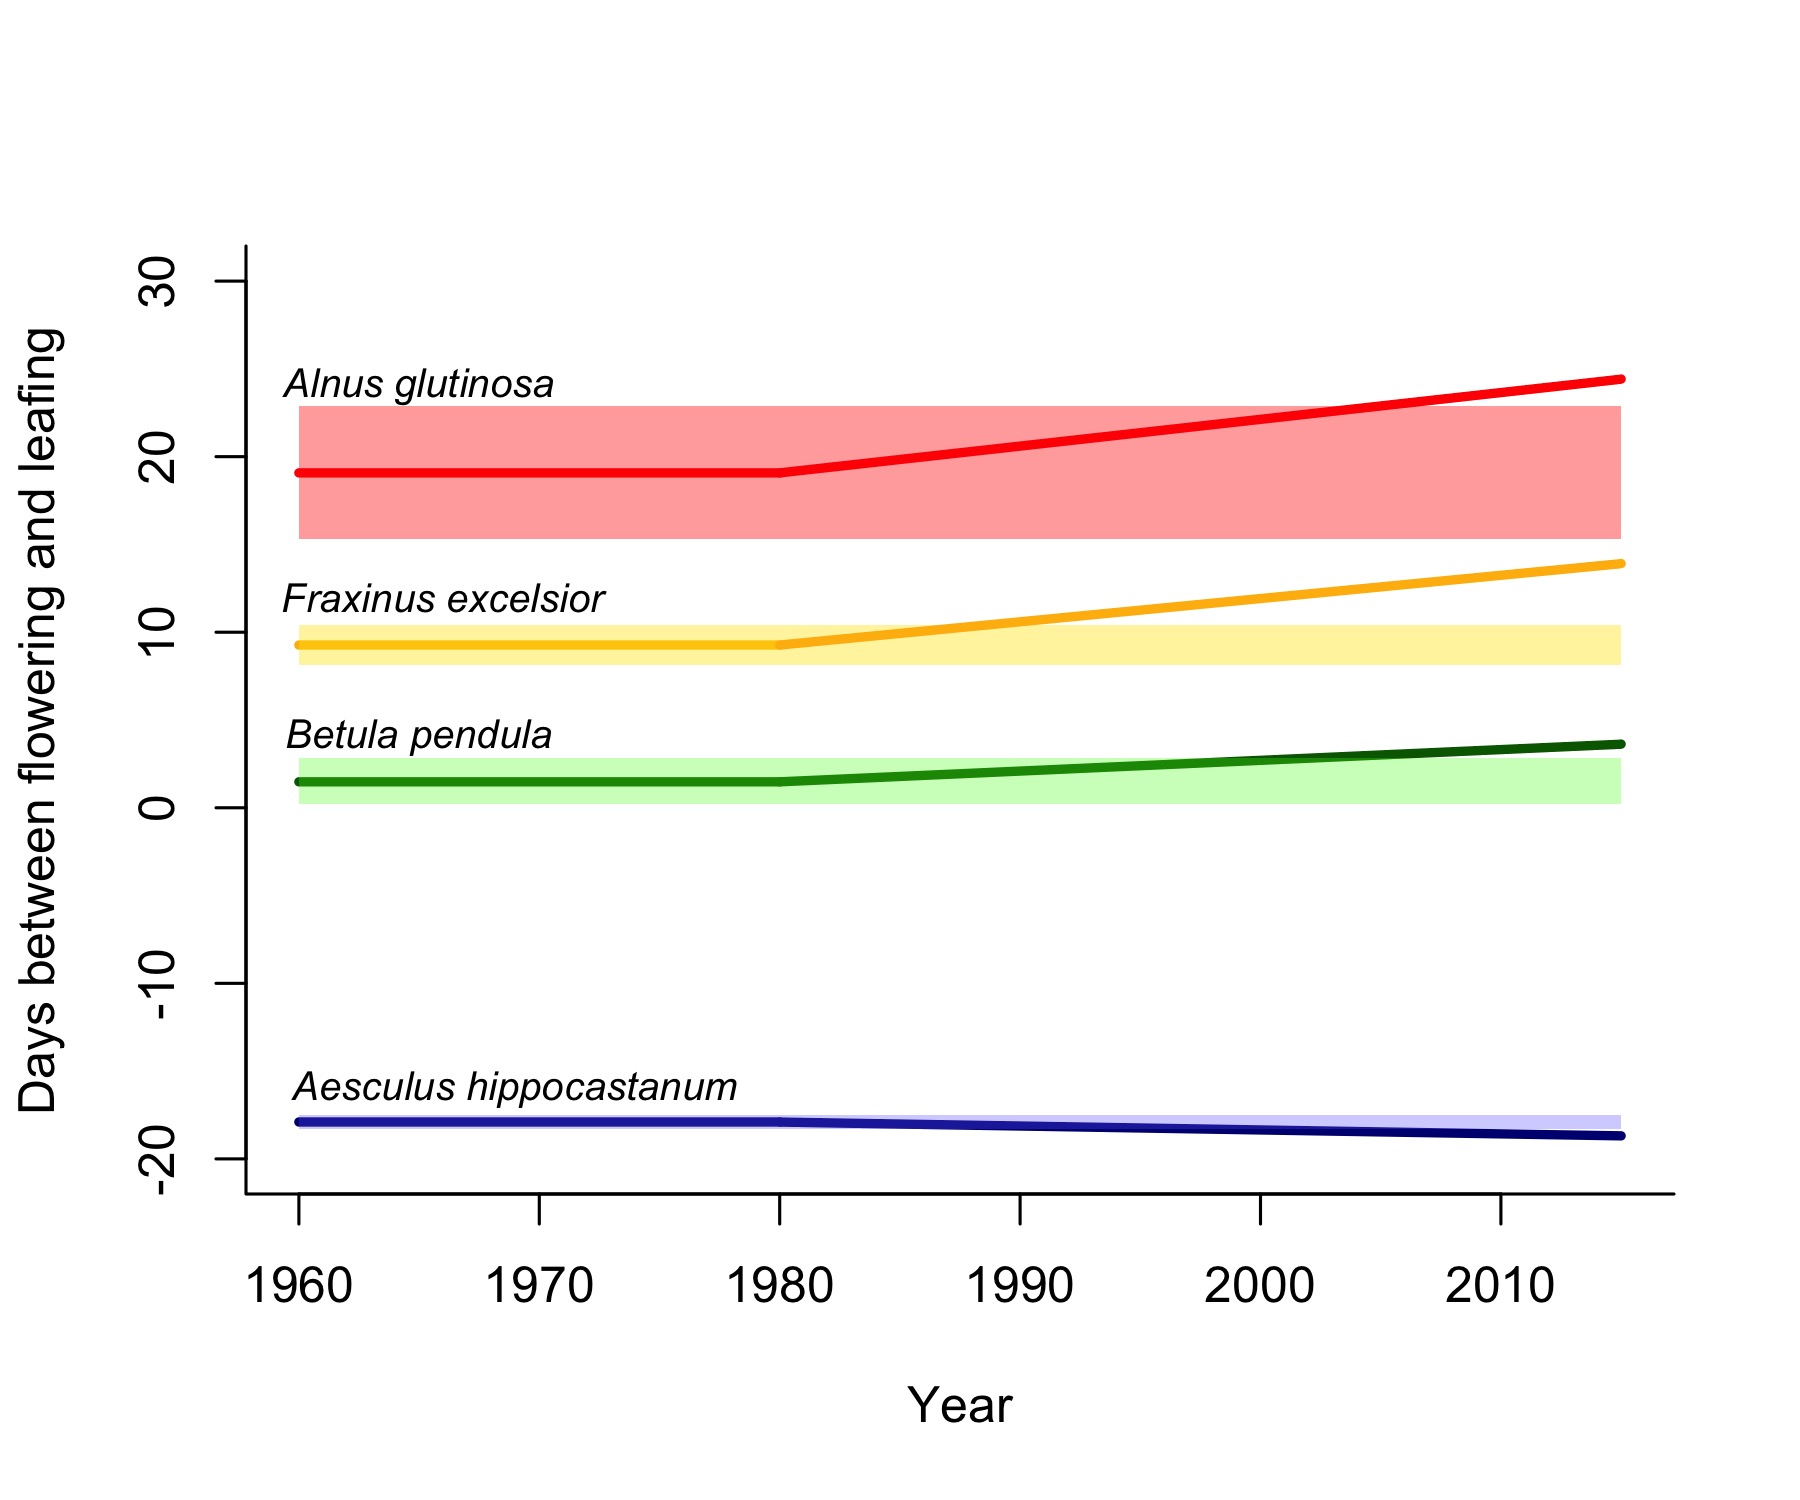
\includegraphics[width=\textwidth]{..//PEP725/FLS_climate_change.jpeg} 
    \caption{\textbf{FLSs across Europe for four tree species from 1960 to 2015 suggests climate change has generally increased the time between flowering and leafing}, but the direction and rate of change differs across species, which may exacerbate fitness differences within forest communities. To detect the effect of climate change on average FLS, we used models that allow for shifts in FLS after 1980. Lines represent the mean trend in FLS per species, and the highlighted regions indicate historic range of FLS variability (95\% credible intervals of the pre-1980 average) from the PEP725 database \citep{PEP725}.}
    \label{fig:climchange}
\end{figure}

  \begin{figure}[ht]
    \centering
    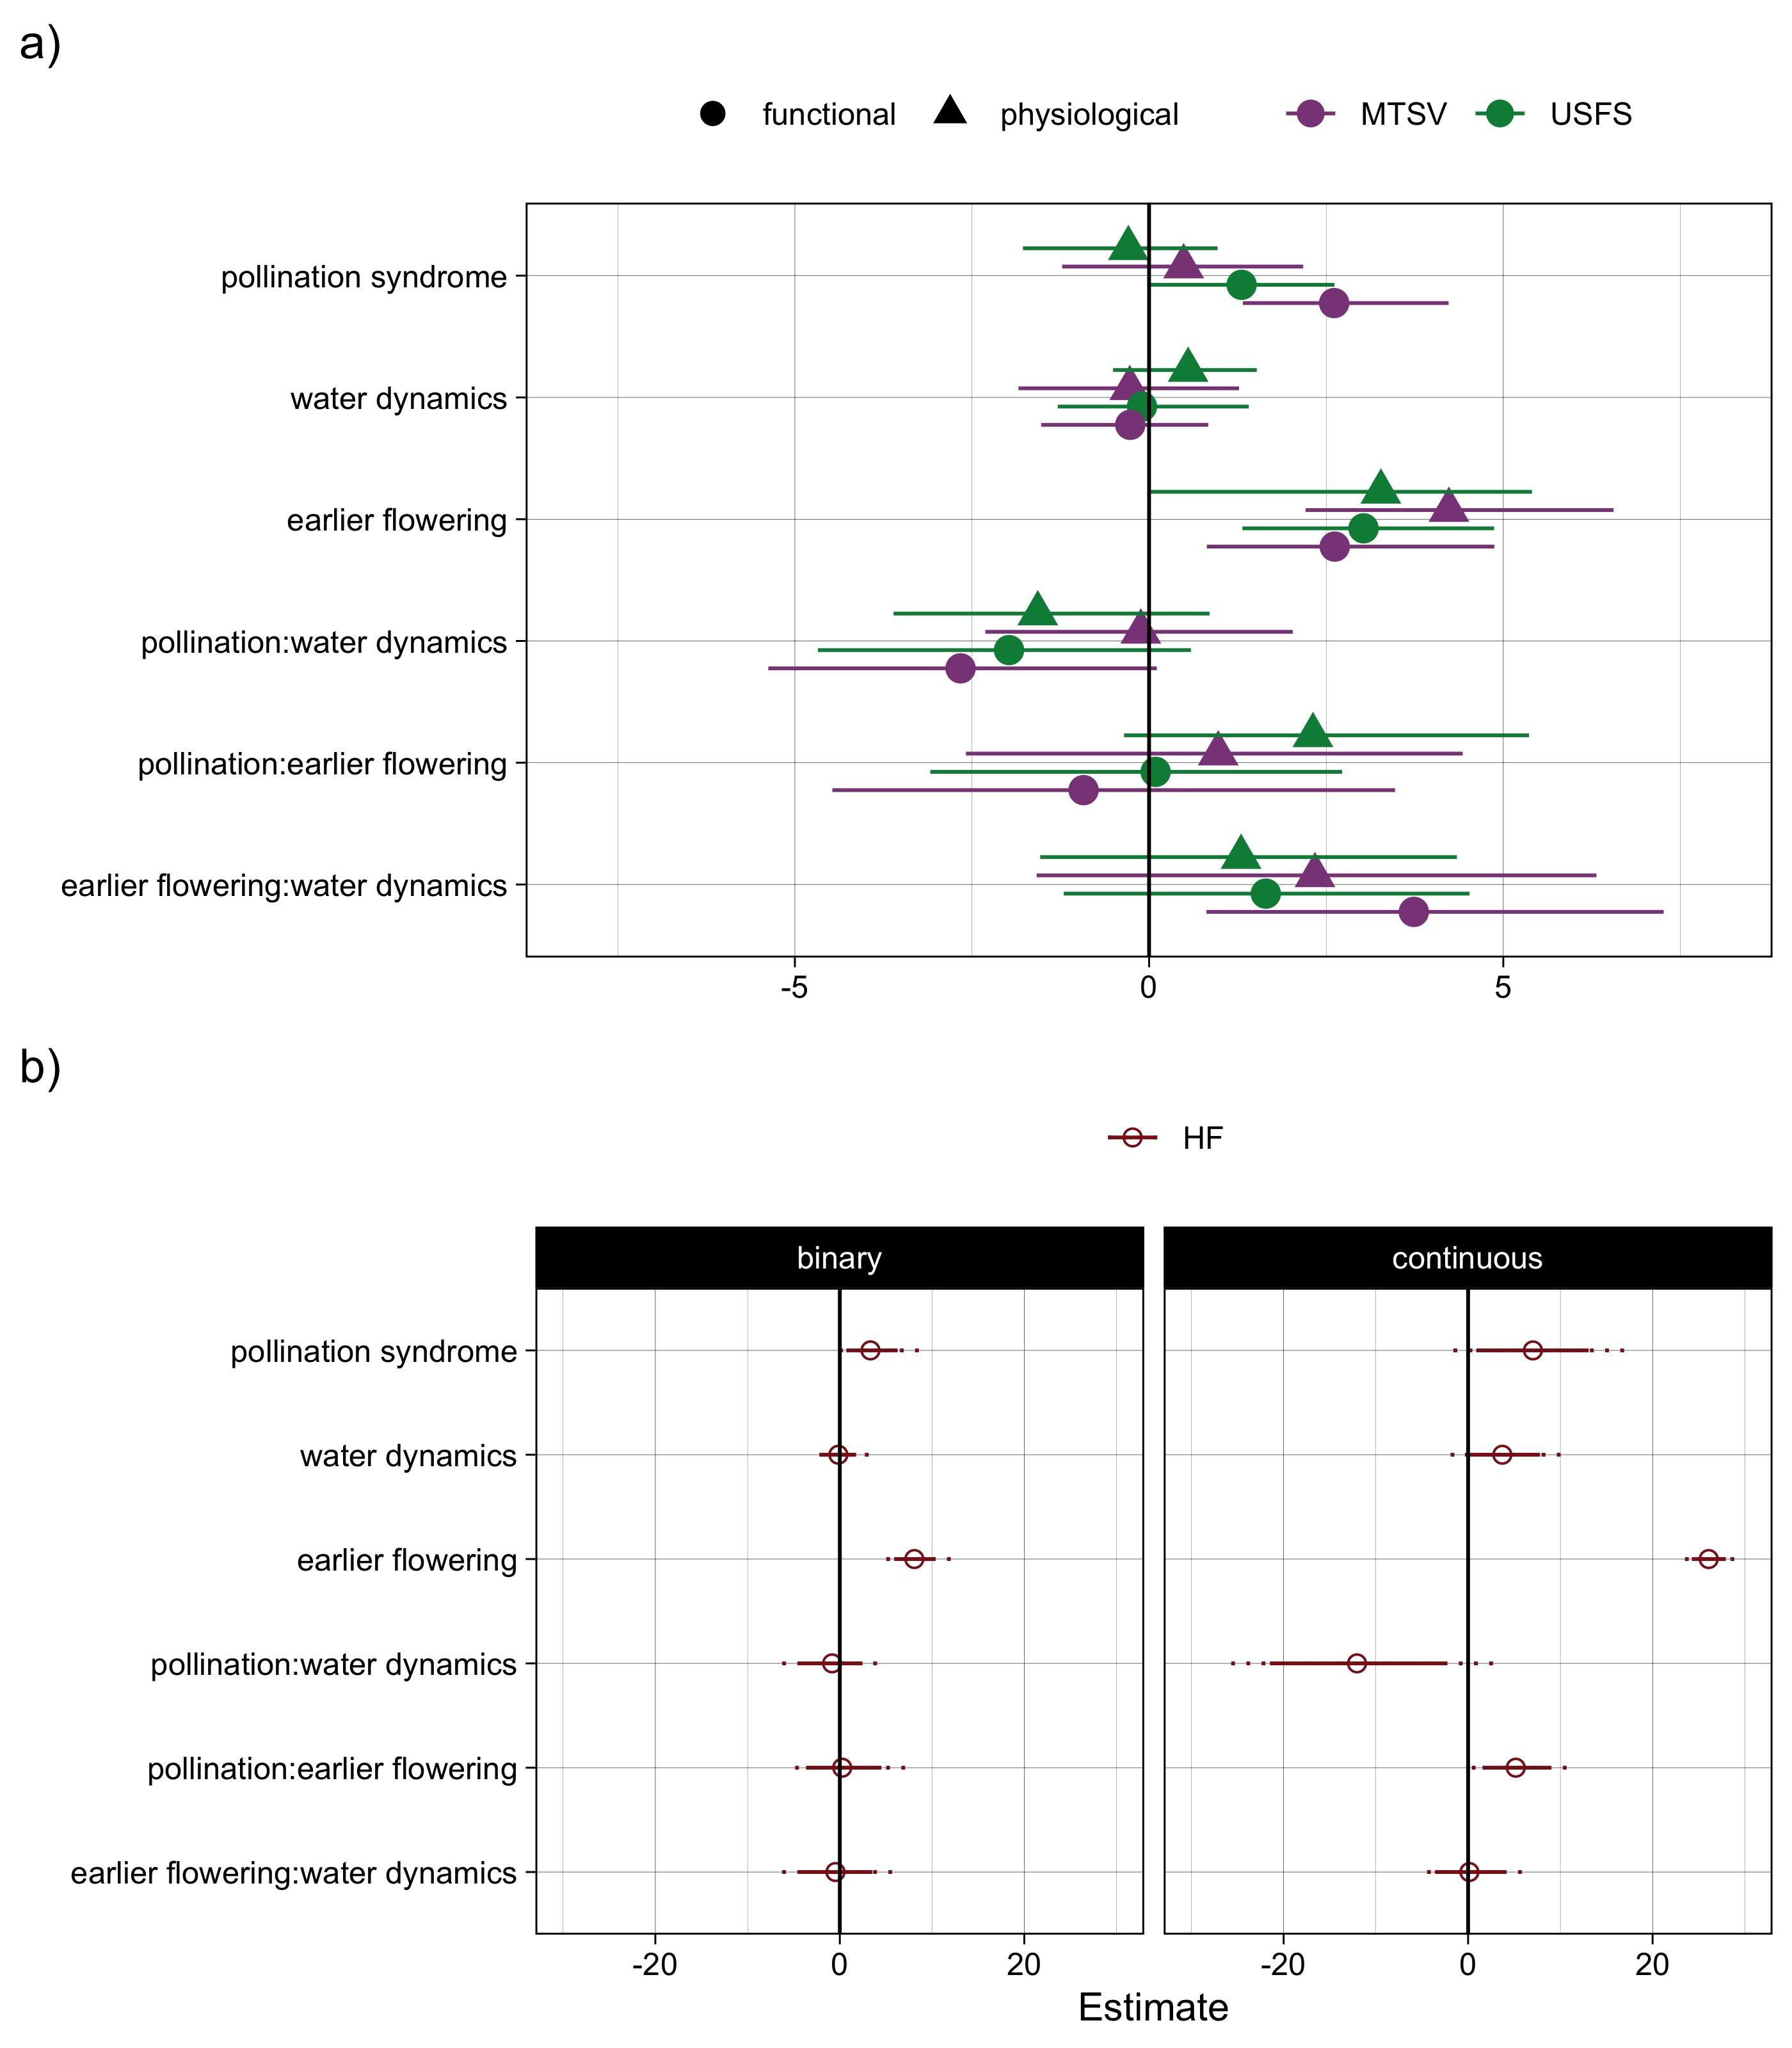
\includegraphics[width=\textwidth]{..//muplots.jpeg}
    \caption{\textbf{Estimated effects of water dynamics (minimum precipitation across species range), pollination syndrome, and earlier flowering time on FLS patterns across three case studies.} We used phylogenetic adjustments and standardized units to make a basic comparison of datasets of different  definitions of of FLS and  data types (categorical and continuous).  }
  \label{fig:muplots}
    \end{figure}

%\begin{figure}[ht]
 %   \centering
%    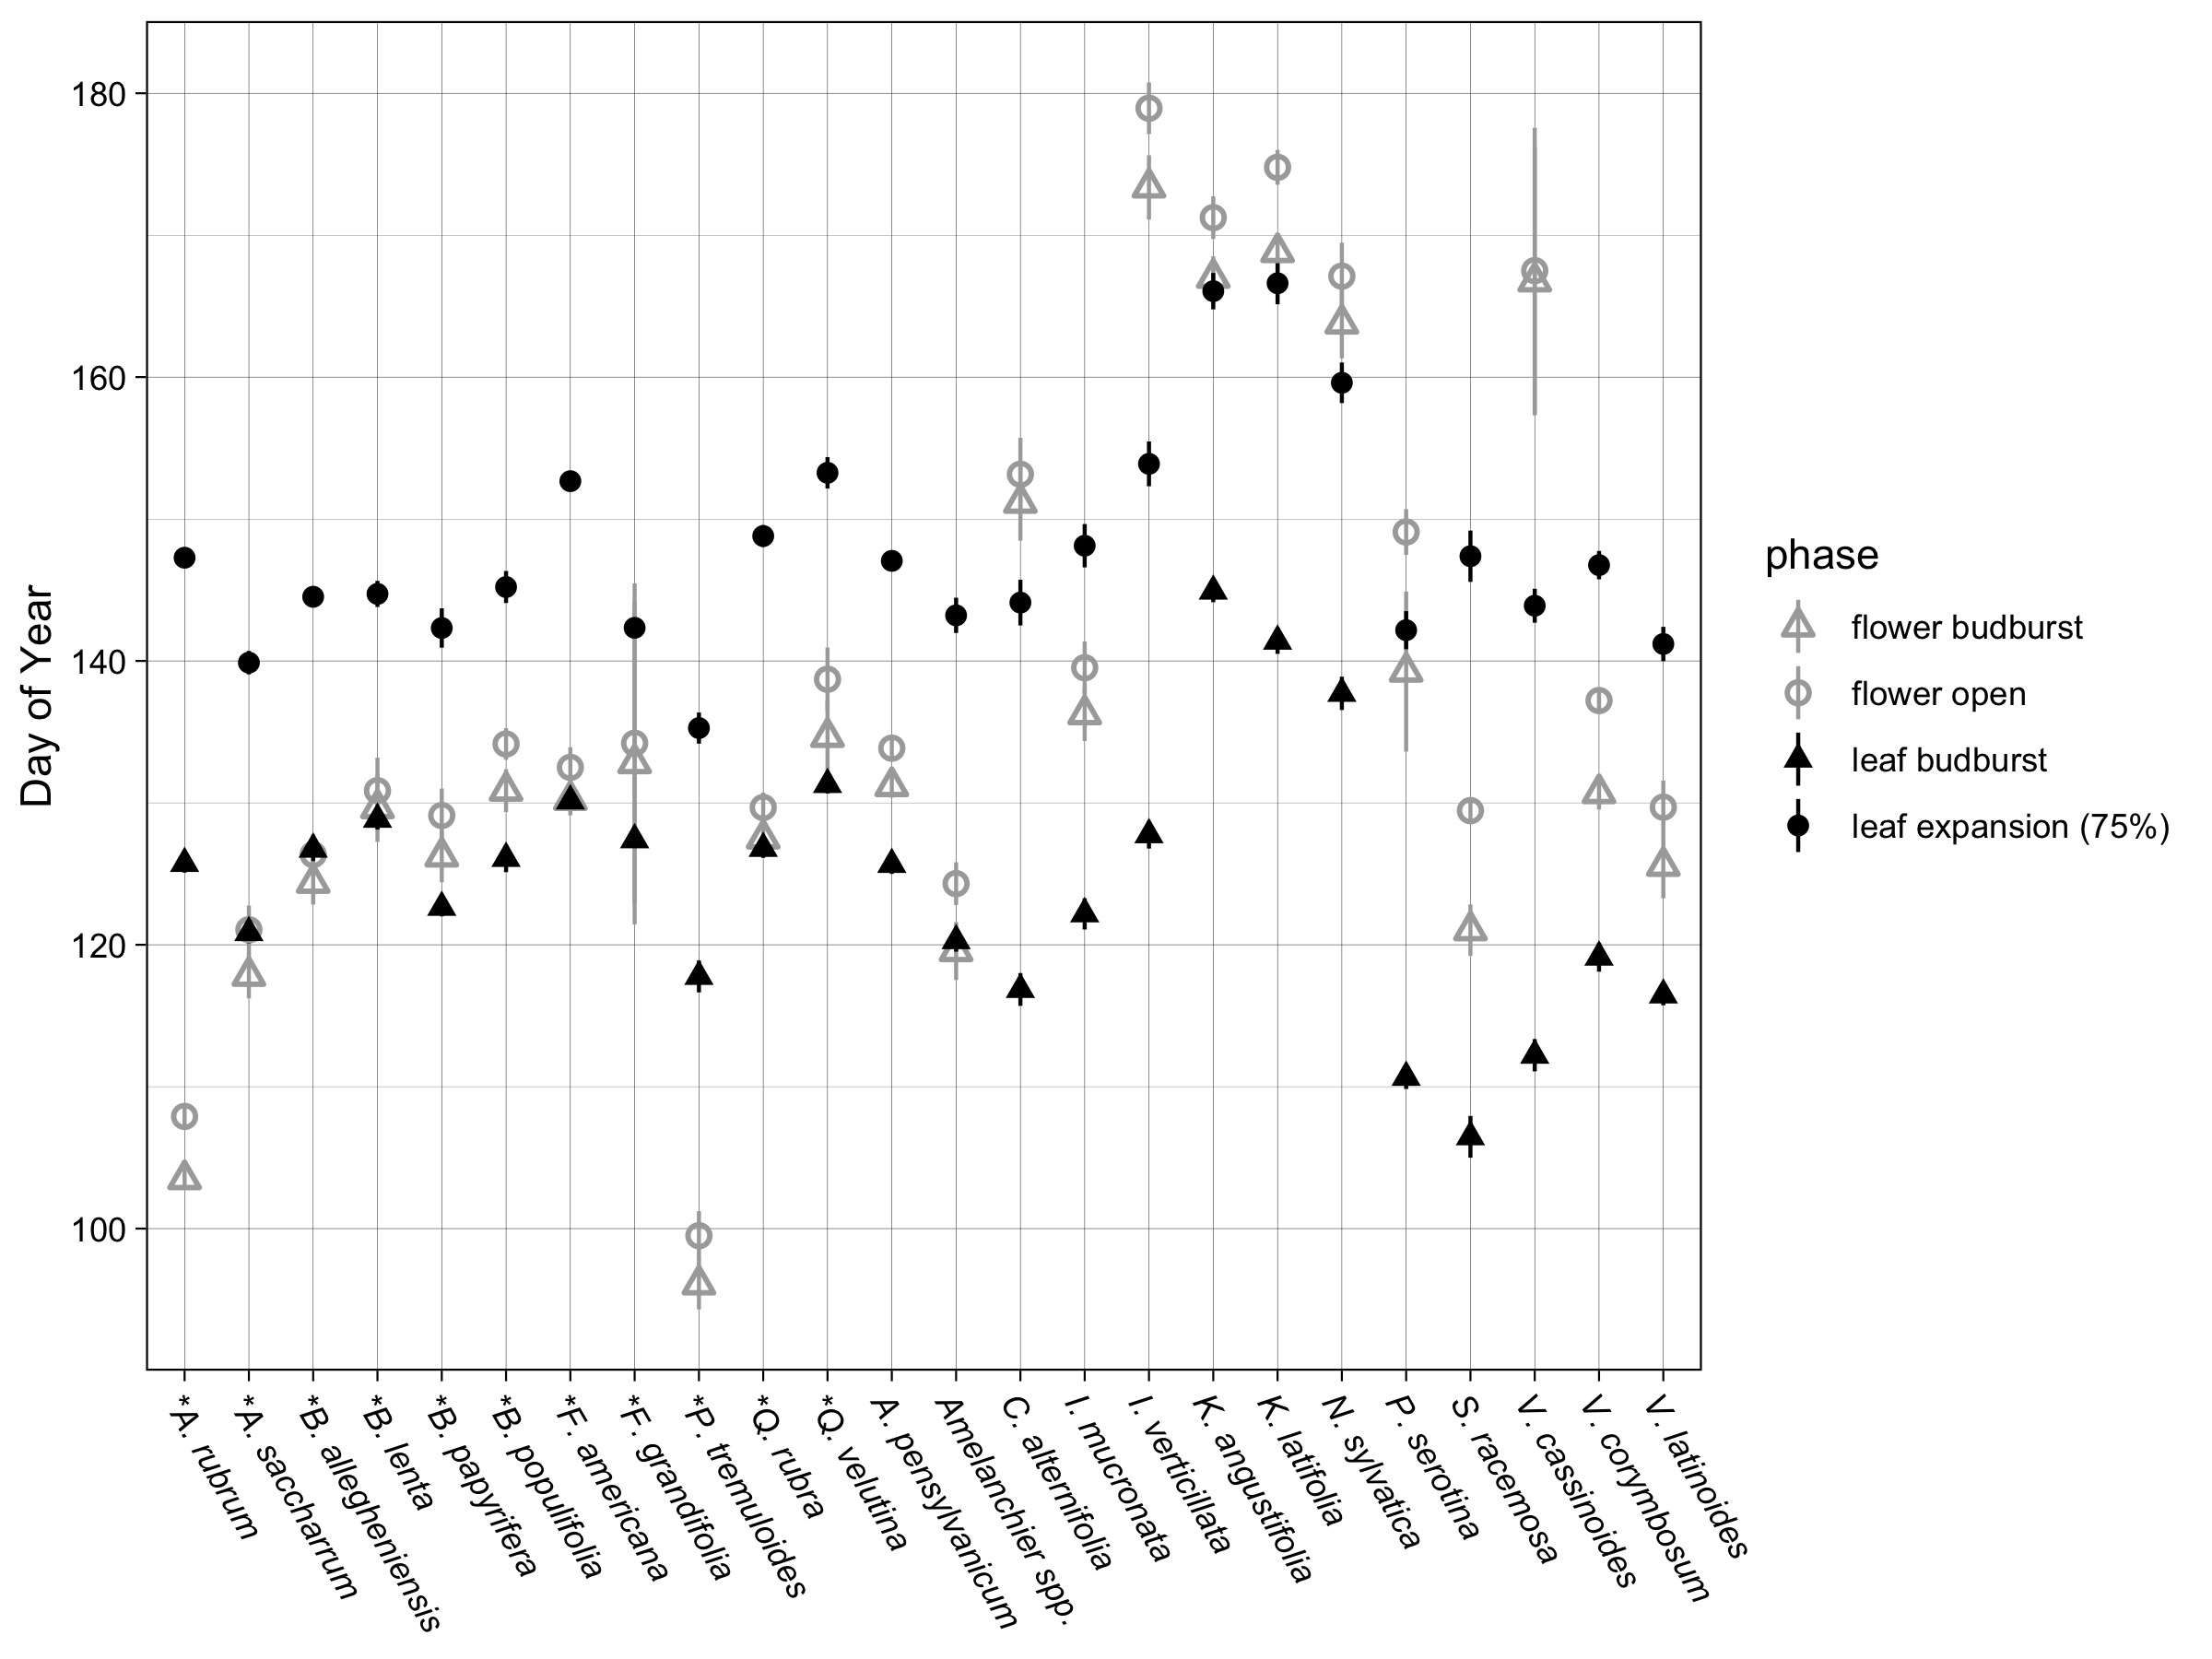
\includegraphics[width=\textwidth]{..//HarvardForest/HFmeans_expanded.jpeg}
 %   \caption{\textbf{Average inter-specific FLS variation at Harvard Forest, MA from 1990-2015.} This community displays all major FLS patterns, but because of overlapping floral and vegetative sub-phases and interannual variability in phenology (lines indicate standard error for each phenophase mean), it is difficult to neatly assign all species to a FLS category. Other notable patterns relevant to the FLS hypotheses can be seen. 1) As predicted by the early flowering hypothesis, the earliest species to initiate spring phenology are hysteranthous. 2) As predicted by the pollination syndrome hypothesis, wind-pollinated species (indicated with a *) may vary in whether their flowers or vegetative buds break first, but all open their flowers before leaves expand to 75\%.}
  %  \label{fig:HFmeans}
%\end{figure}

 \begin{figure}[ht]
        \centering
          
\includegraphics[width=\textwidth]{..//HarvardForest/HF_Q_ru_interannual.jpeg}
          \caption{\textbf{Individual FLS variability over time for \textit{Quercus rubra} at Harvard Forest.} While this species is typically is classified as synanthous, we see here that the the order of flower and leaf bud break, and the time between these events varies considerably for each individual over time, and between individuals in any given year. None of this variation can be accounted for in a categorical FLS classification system.}
        \label{fig:Quercus}
    \end{figure}
    

 \begin{figure}[ht]
        \centering
          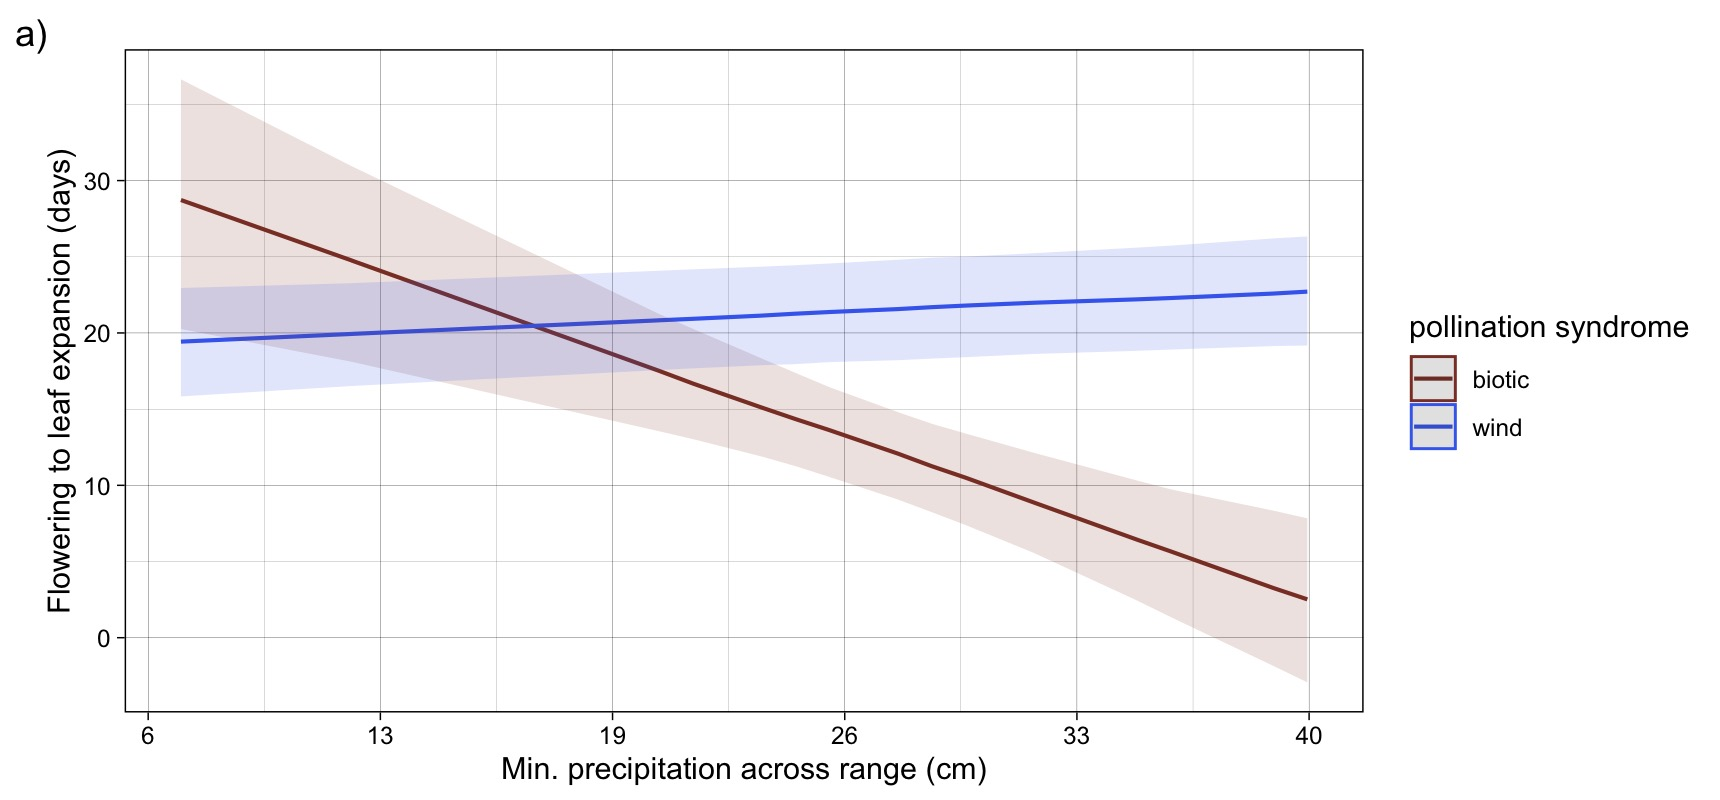
\includegraphics[width=\textwidth]{..//HarvardForest/apcs.jpeg}
           \caption{\textbf{Average predictive comparisons suggest that water dynamics may be a driver of hysteranthy in biotically-pollinated but not in wind-pollinated taxa, suggesting future work on FLS must accommodate overlapping hypotheses.} For species flowering in mid-May (the 25 year community average) these systematic differences}
        \label{fig:apcs}
    \end{figure}
\end{document}